\documentclass[12pt]{article}

% Versão em português (pt-BR) de main.tex. Mantenha as duas versões em
% sincronia: mesmas seções, rótulos, tabelas, figuras, números e citações.

\usepackage{sbc-template}

\usepackage{graphicx,url}

\usepackage[english,brazilian]{babel}
\usepackage[utf8]{inputenc}
\usepackage[T1]{fontenc}

\usepackage{float}
\usepackage{array}

\sloppy
\setlength{\belowcaptionskip}{6pt}

% Nota de acesso das referências online (refs.bib usa \bibaccessed; main.tex
% fica com o padrão em inglês definido no próprio campo note).
\newcommand{\bibaccessed}{Acesso em: nov. 2026}

\title{Um Juiz Online com Feedback Guiado por IA\\para o Ensino Introdutório de Programação}

\author{Juan Israel dos Anjos, Suelen Mapa de Paula}

\address{Instituto Federal de Educação, Ciência e Tecnologia de Minas Gerais
  (IFMG)\\
  Rua Afonso Sardinha, 90, Bairro Minas Talco\\
  Ouro Branco/MG – CEP: 36494-018 – Brasil
  \email{juaniwk3@gmail.com, suelen.mapa@ifmg.edu.br}
}

\begin{document}

\maketitle

\begin{otherlanguage}{english}
\begin{abstract}
  Online judges give novice programmers immediate correction, but they were designed for contests: a failed submission returns a bare verdict such as ``Wrong Answer'', and teachers find them hard to adapt to coursework. This paper asks how an online judge can be designed to support the teaching of introductory programming, and how novices perceive it in class. Following a design-based research approach, we built WhyRunner, an educational judge that combines teacher-curated lessons, feedback that keeps hidden tests confidential, and AI hints instructed to explain the error without giving the fix. In a first classroom use, 30 first-year technical high-school students, 24 of whom had never used a judge, solved an exercise list; the mean System Usability Scale score was 72.1, above the benchmark of 68, the AI hints were the feature students valued most, and exact output matching was the main obstacle. The evidence is limited to students' perceptions in one lesson.
\end{abstract}
\end{otherlanguage}

\begin{resumo}
  Juízes online dão correção imediata a programadores iniciantes, mas foram projetados para competições: uma submissão com falha devolve apenas um veredito como ``Resposta Errada'', e professores têm dificuldade em adaptá-los às atividades da disciplina. Este artigo investiga como um juiz online pode ser projetado para apoiar o ensino introdutório de programação e como iniciantes o percebem em sala. Seguindo uma abordagem de pesquisa baseada em design, construímos o WhyRunner, um juiz educacional que combina aulas curadas pelo professor, feedback que preserva o sigilo dos casos de teste ocultos e dicas de IA instruídas a explicar o erro sem entregar a correção. Num primeiro uso em sala, 30 alunos do primeiro ano do ensino médio técnico, 24 dos quais nunca tinham usado um juiz, resolveram uma lista de exercícios; a nota média na System Usability Scale foi 72,1, acima da referência de 68, as dicas de IA foram o recurso mais valorizado e a comparação exata da saída foi o principal obstáculo. A evidência se limita à percepção dos alunos em uma aula.
\end{resumo}

\section{Introdução}

A avaliação automática de exercícios de programação é comum em disciplinas introdutórias \cite{alamutka2005survey,ihantola2010review}, e os juízes online, que executam o programa submetido contra casos de teste predefinidos e devolvem um veredito, são sua forma mais difundida \cite{wasik2018survey}. Para o iniciante, a imediatez dessa correção é valiosa, mas seu conteúdo é pobre: a maioria dos juízes foi construída para competições, em que a justiça exige que uma submissão com falha receba apenas um veredito como ``Resposta Errada'' ou ``Tempo Limite Excedido''. A pesquisa sobre feedback mostra que ele favorece a aprendizagem quando diz ao aprendiz onde ele está e como prosseguir \cite{hattie2007power}, e revisões sobre feedback automático em programação constatam que a maioria das ferramentas informa \emph{se} um programa está errado, e não \emph{por quê} \cite{keuning2018systematic}. Os professores, por sua vez, acham os juízes de competição rígidos quando querem passar uma lista ordenada, acompanhar cada aluno ou exigir uma abordagem específica.

Os grandes modelos de linguagem (LLMs) tornaram barato o feedback explicativo, e ferramentas como o CodeHelp \cite{liffiton2023codehelp} e o CodeAid \cite{kazemitabaar2024codeaid} mostraram que um assistente pode ser restringido a ajudar sem escrever a solução. Esses assistentes, porém, ficam fora do juiz: não veem o teste que falhou, e um juiz que simplesmente repassasse seu relatório de falha aos alunos revelaria os testes ocultos que mantêm a correção honesta. O problema tratado aqui é, portanto, como levar feedback guiado e explicativo \emph{para dentro} do ciclo de correção do juiz em sala, sem entregar respostas nem testes, e de uma forma que o professor possa organizar.

\textbf{Pergunta de pesquisa.} \emph{Como um juiz online pode ser projetado para apoiar o ensino introdutório de programação, e como alunos iniciantes percebem esse juiz em uma turma real?} Ela se divide em duas subperguntas: (QP1) quais escolhas de projeto adaptam um juiz de competição ao ensino em sala, e (QP2) como iniciantes percebem sua usabilidade e seu feedback, incluindo as dicas de IA, em um primeiro uso em sala.

\textbf{Contribuições.} (1) Um conjunto de princípios de projeto para um juiz educacional, derivados da literatura e de um uso exploratório, e sua realização no WhyRunner: aulas curadas pelo professor com boletim e modos visuais de resposta, vereditos e relatórios de falha filtrados para preservar o sigilo dos testes ocultos, e dicas de IA instruídas a explicar o erro sem entregar a correção (\S\ref{sec:design}). (2) Uma implementação cuja correção técnica foi verificada com uma suíte de benchmarks reproduzível (\S\ref{sec:validation}). (3) Uma primeira avaliação em sala com 30 alunos iniciantes, relatando usabilidade, utilidade percebida do feedback e os obstáculos encontrados, junto com as mudanças que esses obstáculos motivaram (\S\ref{sec:evaluation-status}).

\section{Trabalhos Relacionados}\label{sec:related}

\textbf{Juízes online e avaliação automática.} Levantamentos traçam a avaliação automática de programação ao longo de várias décadas e classificam as ferramentas pelo que verificam e por como relatam o resultado \cite{alamutka2005survey,ihantola2010review,wasik2018survey}. Sistemas de competição como o \textbf{DOMjudge} \cite{domjudge2024} e o \textbf{BOCA} \cite{de2004boca}, sistema das etapas regionais brasileiras da ICPC, priorizam robustez e justiça: as equipes recebem vereditos e os dados de teste permanecem ocultos. Várias plataformas acrescentam uma camada de ensino. O \textbf{beecrowd} (antigo URI Online Judge) oferece um grande banco de problemas e um módulo Academic em que professores criam turmas e listas de exercícios e acompanham o progresso dos alunos \cite{bez2014uri}. O \textbf{Run.codes} \cite{runcodes2024}, desenvolvido por universidades brasileiras, permite ao professor criar listas e competições em várias linguagens e se integra a ambientes virtuais de aprendizagem. O \textbf{CodeRunner} \cite{lobb2016coderunner} é um tipo de questão do Moodle em que o professor cria questões de programação corrigidas por testes dentro de questionários. Protótipos acadêmicos próximos ao nosso incluem o \textbf{Ataux} \cite{silva2021ataux}, que organiza turmas resolvendo listas pelo Codeforces e teve a usabilidade avaliada com 71 alunos, e o \textbf{GOJ} \cite{lima2022gamma}, que corrige problemas de maratonas passadas da UnB. Em todos eles, o feedback de uma submissão com falha é o veredito e, no máximo, os dados de teste que o autor decidiu mostrar.

\textbf{Feedback com IA no ensino de programação.} Os LLMs mudaram o que o feedback automático pode ser \cite{denny2024computing}: podem reescrever mensagens de erro obscuras do compilador em explicações que iniciantes acham mais claras \cite{leinonen2023error}, e assistentes já foram implantados em disciplinas reais com salvaguardas contra a entrega de código. O CodeHelp \cite{liffiton2023codehelp} responde a perguntas dos alunos sobre seu código com explicações e se recusa a escrever a solução; o CodeAid \cite{kazemitabaar2024codeaid}, implantado em uma turma grande, também evita soluções diretas e foi avaliado com alunos e educadores. Feedback com IA para programação, portanto, não é novidade. O que o WhyRunner acrescenta é sua posição dentro do juiz: a dica é pedida sobre uma submissão específica que falhou, o modelo vê o teste que falhou mesmo quando o aluno não pode vê-lo, a dica se adapta ao modo de resposta (código, blocos ou Parsons) e o organizador de uma competição limita quanta ajuda é permitida. A Tabela~\ref{tab:judge-comparison} resume a comparação.

\begin{table}[ht]
\centering
\scriptsize
\setlength{\tabcolsep}{3pt}
\caption{Comparação do WhyRunner com ferramentas relacionadas, conforme descritas nas fontes citadas. n/r: não relatado nessas fontes; ---: não se aplica.}
\label{tab:judge-comparison}
\resizebox{\textwidth}{!}{%
\begin{tabular}{lccccccccc}
\hline
\textbf{Recurso} & \textbf{DOMjudge} & \textbf{BOCA} & \textbf{beecrowd} & \textbf{Run.codes} & \textbf{CodeRunner} & \textbf{Ataux} & \textbf{GOJ} & \textbf{CodeHelp} & \textbf{WhyRunner} \\
\hline
Corrige código por testes            & Sim & Sim & Sim & Sim & Sim & Sim$^a$ & Sim & Não & Sim \\
Listas curadas e acompanhamento      & Não & Não & Sim & Sim & Sim$^b$ & Sim & Não & Não & Sim \\
Competições com placar ao vivo       & Sim & Sim & Sim & Sim & Não & n/r & n/r & Não & Sim \\
Feedback explicativo (LLM)           & Não & Não & n/r & Não & Não & Não & Não & Sim & Sim \\
Feedback vê o teste que falhou       & --- & --- & --- & --- & --- & --- & --- & Não & Sim \\
Modos visuais (blocos, Parsons)      & Não & Não & n/r & Não & n/r & Não & Não & --- & Sim \\
Abordagem exigida (restrições)       & Não & Não & n/r & n/r & n/r & Não & Não & --- & Sim \\
\hline
\multicolumn{10}{l}{$^a$ via Codeforces. $^b$ como questionários dentro do Moodle.}
\end{tabular}}
\end{table}

\section{Metodologia}\label{sec:methodology}

O trabalho segue a pesquisa baseada em design, na qual uma intervenção para um problema educacional real é projetada, posta em prática em um contexto autêntico e refinada a partir do que essa prática revela \cite{wang2005dbr}. Ele teve três fases.

\textbf{(1) Análise do problema e princípios de projeto.} A literatura acima, a experiência do autor com plataformas de competição e conversas informais com alunos e professores apontaram três lacunas: feedback restrito ao veredito, pouco controle do professor sobre as atividades da disciplina e interfaces voltadas a competições. Uma versão exploratória foi então usada informalmente por cinco colegas, sem roteiro nem questionário; suas queixas confirmaram as lacunas e viraram mudanças (\S\ref{sec:implementation}). Os princípios resultantes são apresentados com o projeto na \S\ref{sec:design}.

\textbf{(2) Desenvolvimento e validação técnica.} O WhyRunner foi desenvolvido de forma iterativa. Como um feedback errado ou que vaze testes comprometeria qualquer uso no ensino, sua correção foi verificada com testes automatizados e uma suíte de benchmarks reproduzível antes do uso em sala (\S\ref{sec:validation}).

\textbf{(3) Avaliação em sala.} \emph{Contexto e participantes:} uma turma do primeiro ano do curso Técnico em Informática integrado ao ensino médio do IFMG, em 29 de outubro de 2026; os alunos resolveram uma aula com dois problemas em Python durante uma aula regular, com o desenvolvedor presente. \emph{Instrumentos:} o instrumento de avaliação está embutido no sistema: ao fim de uma competição ou aula, os participantes são convidados a um questionário (com elegibilidade verificada no servidor), com termo de consentimento livre e esclarecido, a System Usability Scale (SUS) \cite{brooke1996sus}, itens Likert específicos da atividade e perguntas abertas; uma página restrita ao pesquisador resume e exporta as respostas anônimas. \emph{Análise:} a nota SUS é calculada por respondente e comparada com a referência de 68 \cite{sauro2011sus} e com a escala de adjetivos \cite{bangor2009sus}; os itens Likert são resumidos por suas médias; as respostas abertas foram agrupadas em temas, contando-se as menções de cada tema \cite{braun2006thematic}; para a queixa mais frequente, as submissões armazenadas foram inspecionadas para verificar sua causa. O estudo é descritivo: não tem grupo de comparação nem medida pré/pós, e por isso trata de percepção (QP2), não de ganho de aprendizagem.

\section{WhyRunner: Projeto para o Ensino}\label{sec:design}

Cada princípio de projeto abaixo responde a uma das lacunas identificadas na \S\ref{sec:methodology} (QP1).

\textbf{P1. O professor organiza o trabalho, não só competições.}\label{sec:class-lesson-model} Além das competições cronometradas, o WhyRunner tem um modo assíncrono com três entidades: a \emph{Turma}, em que os alunos entram com um código; a \emph{Aula}, uma lista ordenada e curada pelo professor para uma turma, com prazo opcional; e o \emph{Exercício}, um problema existente colocado em uma aula. Os alunos entregam a aula inteira, e o professor a revisa com feedback em texto livre por exercício. Cada exercício vale a fração de casos de teste aprovados, de modo que um programa parcialmente correto recebe nota parcial, e um boletim mostra cada aluno contra cada exercício e pode ser exportado. As competições mantêm as convenções de maratona (número de tentativas, penalidades, primeiro a resolver) pelo papel motivador que competições têm no ensino de informática \cite{audrito2012contests}.

\textbf{P2. Várias portas de entrada para o código.} Seguindo a recomendação de que o ensino de programação comece com ambientes visuais e passe gradualmente ao texto \cite{audrito2012contests,weintrop2015block}, cada exercício tem um modo de resposta: \emph{código}; \emph{blocos}, blocos Blockly convertidos em Portugol, uma pseudolinguagem em português comum em cursos brasileiros, com o código gerado exibido em modo somente leitura como ponte para o texto; ou \emph{Parsons}, linhas embaralhadas da solução do professor a serem ordenadas e indentadas \cite{parsons2006puzzles}. O programa efetivamente corrigido é sempre gerado no servidor, de modo que correção e dicas funcionam da mesma forma em todos os modos.

\textbf{P3. O feedback diz o que falhou sem entregar os testes.}\label{sec:verdicts}\label{sec:test-confidentiality} Uma submissão com falha recebe o veredito de seu primeiro caso reprovado, distinguindo resposta errada, tempo limite, limite de memória, erro de compilação (com a saída do compilador) e erro de execução, e nunca penalizando uma falha do próprio juiz. Os casos de teste são exemplos públicos ou ocultos. Como no BOCA \cite{de2004boca}, o relatório de falha é filtrado conforme quem o vê: em um exemplo, o aluno vê a entrada, a própria saída, a saída esperada e a saída de erro; em um caso oculto, só o veredito, o número do caso e quantos casos passaram. Nas aulas, o professor escolhe quais casos os alunos veem. A saída pode ser comparada exatamente, ignorando espaços em branco, com tolerância numérica ou por um corretor escrito pelo professor para problemas com várias respostas corretas.\label{sec:output-comparison}

\textbf{P4. Dicas de IA explicam o erro, não a correção.}\label{sec:ai-chain} Em uma submissão com falha, o aluno pode clicar em ``Explicar'' (Figura~\ref{fig:workspace}). O modelo recebe o enunciado, o código e o relatório de falha sem filtro, e é instruído a explicar o erro lógico sem dar a correção exata; o relatório em si nunca chega ao aluno, apenas a resposta do modelo. Organizadores de competições limitam a ajuda a um de quatro níveis (\emph{desligada}, \emph{conceito}, \emph{dica}, \emph{localização}), revelados um de cada vez, e as chamadas têm limite de frequência por aluno. Os mesmos modelos ajudam o professor a criar problemas, redigindo uma solução de referência, revisando o enunciado em busca de ambiguidades e casos-limite ausentes e sugerindo tags de tópico; os rascunhos só são mantidos se o professor os salvar.

\begin{figure}[t]
\centering
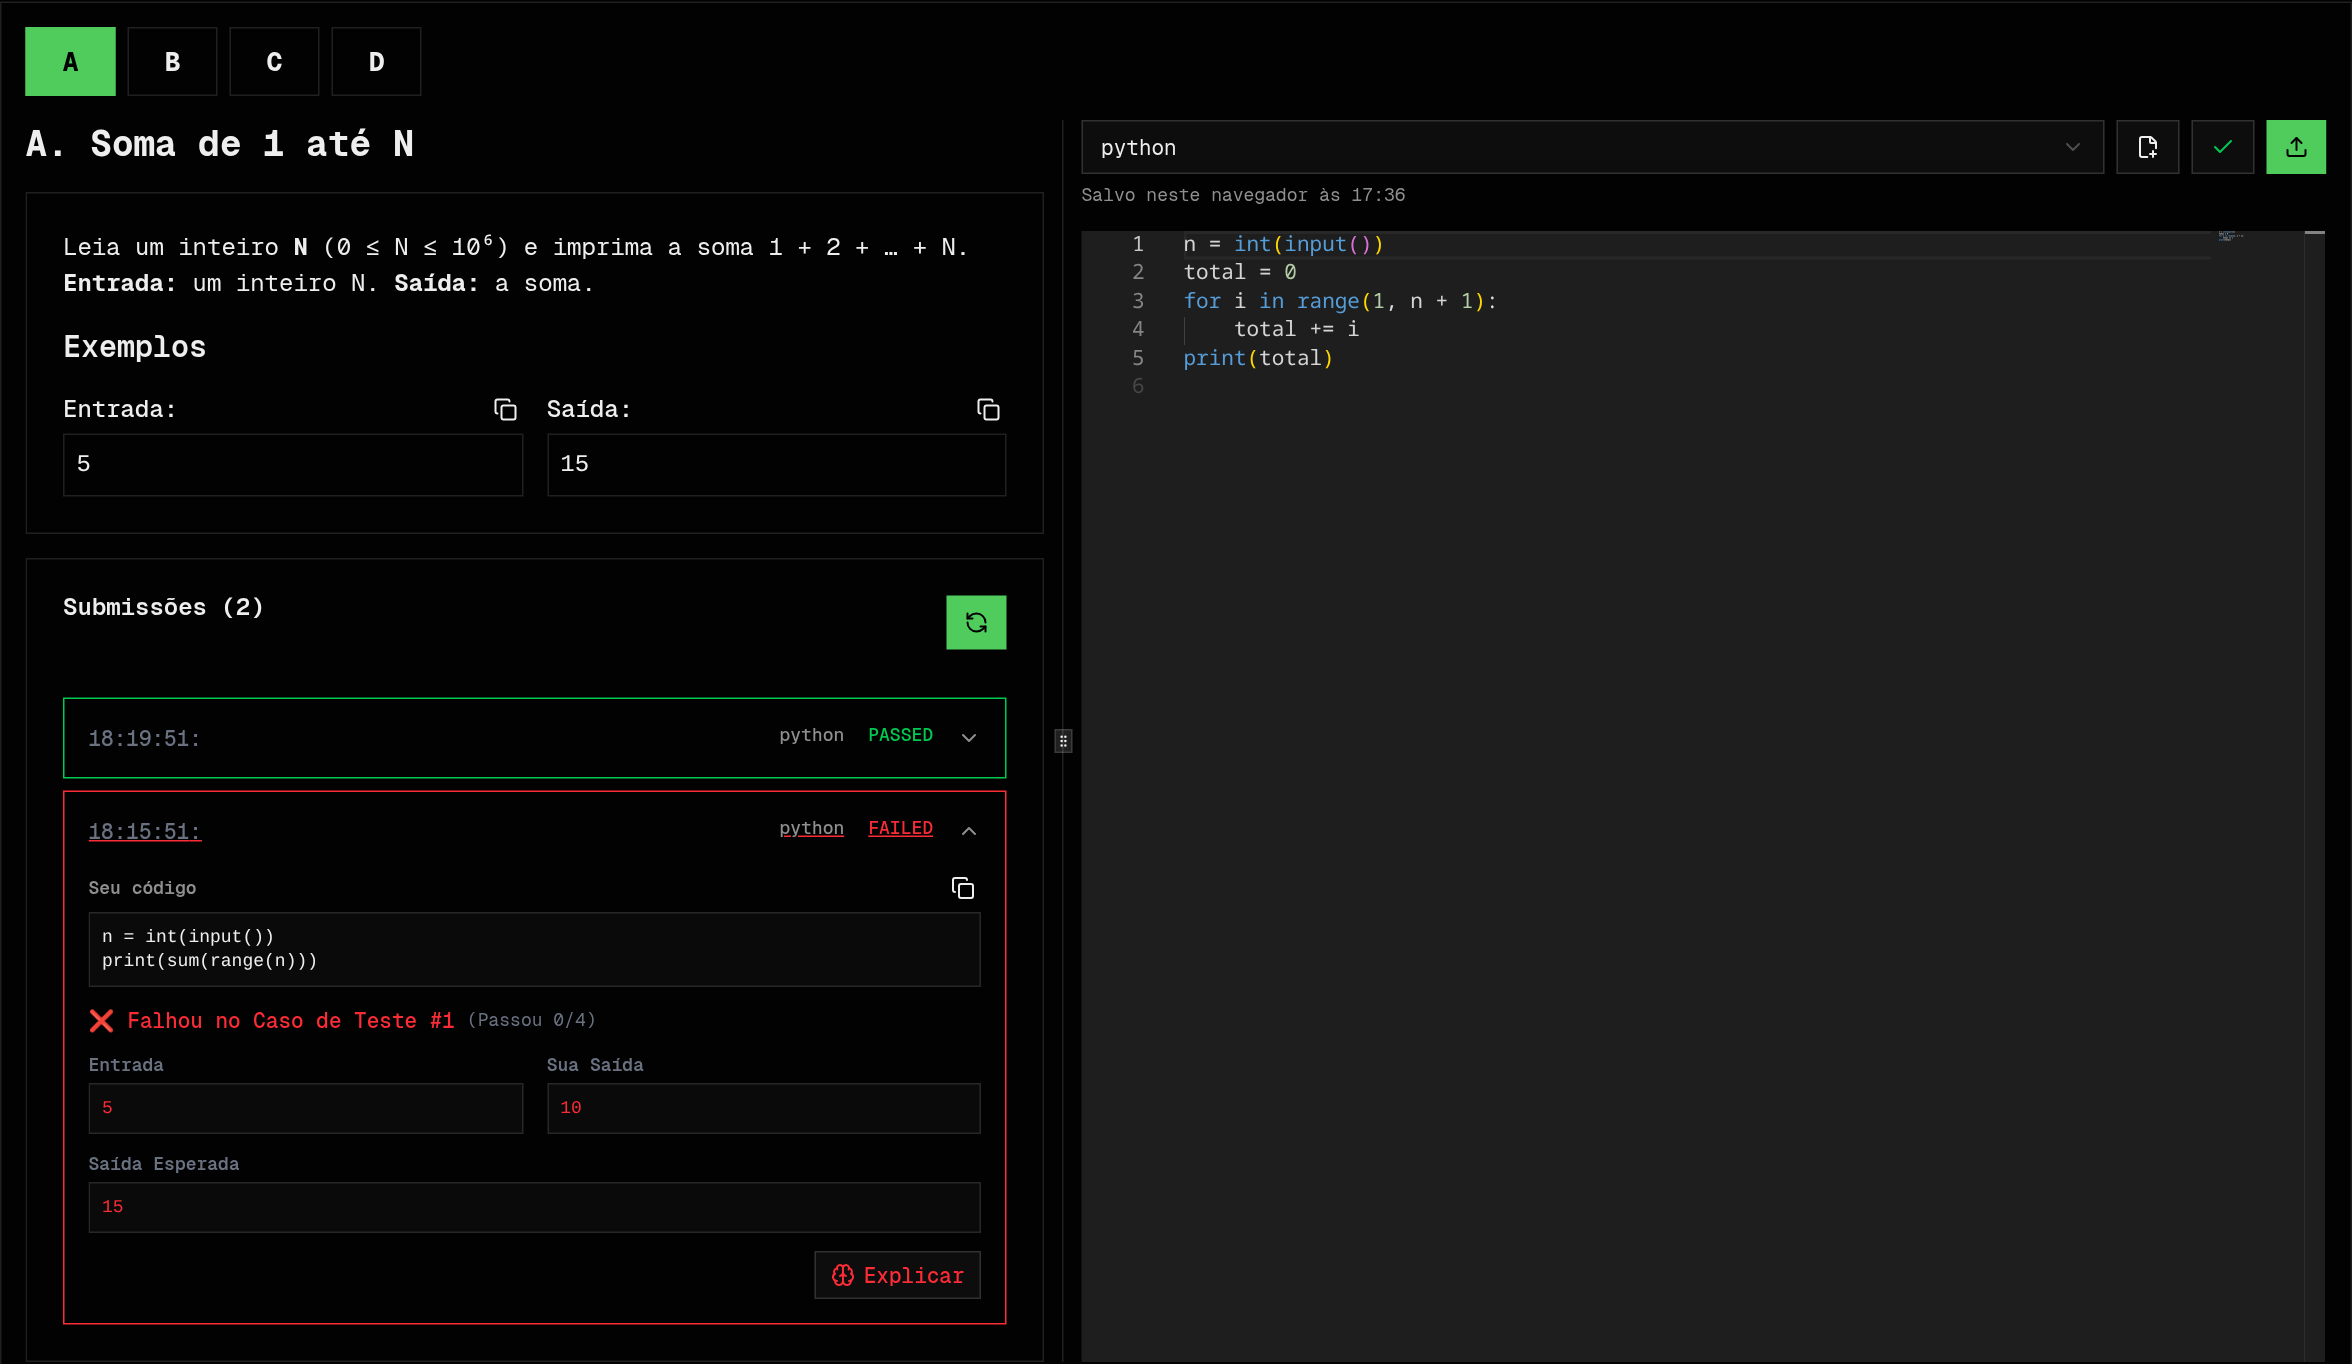
\includegraphics[width=0.8\textwidth]{resolucao.png}
\caption{Ambiente de resolução: enunciado, tentativas com o código submetido e o botão ``Explicar'', e o editor}
\label{fig:workspace}
\end{figure}

\textbf{P5. O professor pode exigir uma abordagem e verificar a honestidade.}\label{sec:prepublish-validation}\label{sec:similarity} O professor pode associar \emph{restrições de solução} a um exercício: regras estruturais (por exemplo, um aninhamento máximo de laços ou uma construção proibida) ou um requisito em texto livre (por exemplo, ``deve usar o algoritmo de Dijkstra'') verificado pelo modelo de linguagem; uma violação nega o crédito mesmo quando todos os testes passam e informa ao aluno qual regra foi quebrada. Antes de um problema ser publicado, sua solução de referência precisa passar nos próprios testes, de modo que os alunos nunca enfrentam um problema com saídas esperadas erradas. Por fim, o dono de uma turma ou competição pode pedir um relatório de similaridade de código baseado em impressões digitais no estilo do MOSS \cite{schleimer2003winnowing}, robusto a renomeação e reformatação; a interface avisa que uma nota alta é motivo para ler os dois programas, não prova de cópia.

\subsection{Implementação}\label{sec:implementation}\label{sec:execution-environment}\label{sec:integration}

O WhyRunner tem dois serviços que compartilham um banco PostgreSQL: uma aplicação web em Next.js, que contém a interface e toda a lógica de negócio, e um worker de correção escrito em Rust que executa cada caso de teste no \texttt{isolate} \cite{mares2012isolate}, o sandbox da Olimpíada Internacional de Informática, sem rede e com limites de tempo, memória e processos. Ele suporta C, C++, Java, Python, Rust e Portugol. As chamadas de IA passam por uma cadeia de modelos (Gemini 3.5 Flash e Flash-Lite \cite{gemini2023}, depois Claude Haiku 5.5 \cite{anthropic2026haiku}), para que a queda de um provedor não desative as dicas.

A arquitetura é fruto de iteração. A fila de submissões passou do Redis ao AWS SQS e, por fim, ao mecanismo de notificação do próprio PostgreSQL, eliminando o broker externo; um backend hospedado e uma API separada deram lugar a um único banco e a ações no servidor; e a execução passou de um contêiner Docker por submissão, que exigia acesso equivalente a root no host, para o \texttt{isolate}. O uso exploratório por cinco colegas gerou três mudanças: cada tentativa mostra o código submetido, um placar no estilo de maratona e erros mais claros na importação de problemas. Uma revisão de segurança da camada web constatou que algumas ações confiavam na entrada do cliente e que os relatórios de falha expunham casos de teste ocultos; ambos foram corrigidos, o que deu origem à filtragem de relatórios de P3.

\section{Validação Técnica}\label{sec:validation}\label{sec:performance}\label{sec:perf-verdicts}\label{sec:perf-similarity}

Os scripts e dados brutos por trás destes números estão no diretório \texttt{bench/} do repositório. Como os alunos agem com base nos vereditos, a correção dos vereditos é o que mais importa: de 72 programas escritos para provocar um dado veredito em seis linguagens, 63 (87,5\%) o receberam, e aceito, resposta errada e tempo limite sempre estiveram certos; as falhas foram os erros do Portugol, corrigidos como resposta errada porque seu executor termina normalmente após imprimi-los, erros de sintaxe do Python corrigidos como erro de execução e uma falha após uma alocação malsucedida. Em variações realistas de saídas corretas, a comparação exata rejeitou 3 de 35 saídas com espaços no fim da linha e 3 de 35 com quebras de linha do Windows, enquanto a comparação que ignora espaços aceitou todas, e nenhum modo aceitou um erro real. O detector de similaridade separou 216 cópias ofuscadas de soluções independentes com AUC ROC de 0,998. O isolamento acrescentou cerca de 5\,ms por execução, e uma rajada de 100 submissões, como quando uma turma inteira submete ao mesmo tempo, foi corrigida em 51\,s por quatro workers em um processador de desktop. Todas as 60 chamadas de IA retornaram uma resposta, 37 delas por um modelo de reserva, com latências medianas de 13--20\,s.

\section{Avaliação em Sala}\label{sec:evaluation-status}

\textbf{Participantes.} Trinta alunos responderam ao questionário logo após a aula, todos em dez minutos. Vinte e quatro nunca tinham usado um juiz online e seis o tinham usado poucas vezes. Não houve competição e nenhum professor respondeu.

\textbf{Usabilidade.} A nota SUS média foi 72,1 (mediana 76,2, DP 18,3, amplitude 22,5--95; IC 95\% de cerca de 65,6--78,6), acima da referência de 68 \cite{sauro2011sus} e na faixa ``boa'' da escala de adjetivos \cite{bangor2009sus}. A dispersão é grande (Figura~\ref{fig:sus-bands}): 13 respondentes tiveram 80,3 ou mais, 4 entre 68 e 80, 8 entre 51 e 67 e 5 abaixo de 51. Integração e facilidade de aprendizado foram os itens mais fortes (Tabela~\ref{tab:sus-items}); os mais fracos diziam respeito à autonomia, à necessidade de suporte (9 de 30 concordaram) e à confiança, o que condiz com uma turma em que 80\% nunca tinham usado um juiz.

\begin{figure}[t]
\centering
\begin{minipage}[c]{0.46\textwidth}
\centering
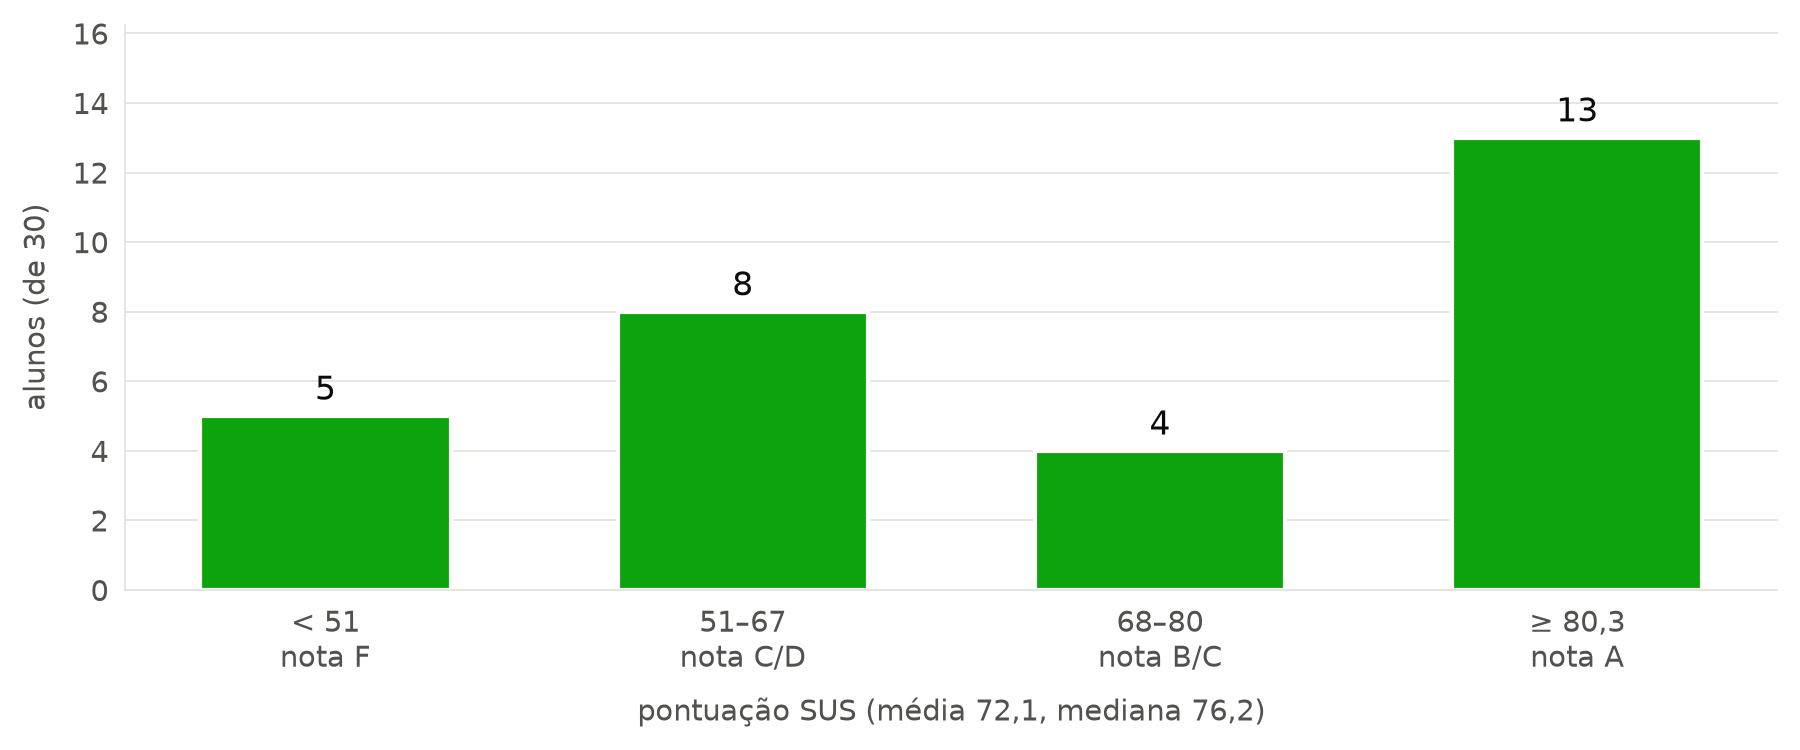
\includegraphics[width=\textwidth]{figures/pt/survey_sus_bands.png}
\caption{Distribuição das notas SUS dos 30 respondentes, por faixa de conceito.}
\label{fig:sus-bands}
\end{minipage}\hfill
\begin{minipage}[c]{0.5\textwidth}
\centering
\scriptsize
\captionof{table}{Resposta média por item da SUS (n = 30, escala 1--5). Nos itens negativos, quanto menor, melhor.}
\label{tab:sus-items}
\begin{tabular}{lr}
\hline
\textbf{Item da SUS} & \textbf{Média} \\
\hline
5. As funções são bem integradas              & 4,13 \\
7. A maioria aprenderia a usá-lo rápido       & 4,07 \\
3. Fácil de usar                              & 3,93 \\
1. Gostaria de usá-lo com frequência          & 3,77 \\
9. Senti-me confiante ao usá-lo               & 3,50 \\
\hline
4. Precisaria de suporte técnico (neg.)       & 2,57 \\
10. Precisei aprender muito antes (neg.)      & 2,13 \\
6. Inconsistência demais (neg.)               & 2,03 \\
8. Complicado de usar (neg.)                  & 1,97 \\
2. Desnecessariamente complexo (neg.)         & 1,87 \\
\hline
\end{tabular}
\end{minipage}
\end{figure}

\textbf{Utilidade percebida do feedback.} O fluxo da turma teve as notas mais altas (Tabela~\ref{tab:survey-items}): 24 de 30 concordaram totalmente que entrar na turma e encontrar a lista foi fácil. Os 23 alunos que usaram as dicas da IA as avaliaram como úteis sem entregar a resposta; o feedback do próprio juiz teve nota menor, e o ganho de confiança foi o item mais baixo. Todos os alunos usaram o editor de código, não os blocos nem o Parsons.

\begin{table}[ht]
\centering
\footnotesize
\caption{Itens específicos da atividade no questionário do aluno para listas de exercícios.}
\label{tab:survey-items}
\begin{tabular}{lrr}
\hline
\textbf{Item (1 = discordo totalmente, 5 = concordo totalmente)} & \textbf{Média} & \textbf{n} \\
\hline
Foi fácil entrar na turma e encontrar a lista             & 4,70 & 30 \\
Ficou claro como entregar a lista                         & 4,43 & 30 \\
Usaria o WhyRunner para estudar sozinho                   & 4,13 & 30 \\
As dicas da IA ajudaram sem entregar a resposta           & 4,04 & 23 \\
O feedback do juiz me ajudou a corrigir meus erros        & 3,53 & 30 \\
O modo de resposta me ajudou a resolver os exercícios     & 3,41 & 29 \\
Sinto-me mais confiante para programar após a lista       & 3,23 & 30 \\
\hline
\end{tabular}
\end{table}

\textbf{Respostas abertas.} O que mais ajudou foi a assistência da IA (cerca de 14 menções, por exemplo, ``as dicas sem entregar a resposta da IA'') e a correção imediata (cerca de 9); todos os sete comentários gerais foram positivos, um deles observando que o sistema ``não mostra resposta, o que é muito bom, pois desenvolve o raciocínio lógico''. A queixa mais frequente (cerca de 9) foi a comparação exata de saída: os dois problemas usavam o modo \emph{exato} e, em um deles, 26 submissões reprovadas de 13 alunos diferiam apenas em espaços em branco e teriam passado na comparação que ignora espaços (12 desses alunos passaram depois). Muitas outras falhas vieram da impressão do prompt do \texttt{input()} do Python. A segunda queixa (cerca de 6) foi não poder ver a própria saída nem o traceback; temas menores incluíram o editor pequeno, o painel de IA sem rolagem e o desejo de executar o código antes de submeter. Um aluno relatou ser surdo e ter achado a atividade um tanto difícil.

\textbf{Mudanças após o teste.} No espírito da pesquisa baseada em design, os obstáculos observados alimentaram uma nova iteração do projeto, integrada em até dois dias (Tabela~\ref{tab:feedback-fixes}). A troca dos problemas existentes para a comparação que ignora espaços foi deixada de fora deliberadamente (\S\ref{sec:limitations}), e uma saída que difere em maiúsculas ou na redação continua sendo rejeitada, já que respeitar a especificação de saída faz parte do que um juiz ensina.

\begin{table}[ht]
\centering
\scriptsize
\caption{Feedback da turma e mudanças resultantes.}
\label{tab:feedback-fixes}
\begin{tabular}{>{\raggedright\arraybackslash}p{5.2cm}>{\raggedright\arraybackslash}p{8.8cm}}
\hline
\textbf{Feedback da turma} & \textbf{Mudança} \\
\hline
Interface abriu em inglês; tradução do navegador quebrou o código inicial; editor pequeno & Português como padrão; código excluído da tradução; tela cheia e tamanho de fonte \\
Número de matrícula digitado como nome de usuário & Etapa de cadastro inicial removida; campo opcional de matrícula \\
Sem a própria saída nem traceback na falha & Entrada, própria saída, saída esperada e saída de erro nos testes visíveis \\
Painel de IA sem rolagem; código apagado ao trocar de linguagem; código colado falhava; prompts do \texttt{input()} impressos & Ajuda com rolagem e acoplável; rascunhos restaurados; caracteres invisíveis normalizados; aviso para imprimir só a saída pedida \\
Não dava para executar antes de submeter & Execução sem correção, com entrada personalizada, no sandbox \\
\hline
\end{tabular}
\end{table}

\textbf{Ameaças à validade.} A avaliação é pequena e descritiva: uma turma, uma lista, uma linguagem e um questionário logo após uma única sessão, sem grupo de comparação nem medida pré/pós, de modo que mostra percepção, não ganho de aprendizagem. Trinta respondentes dão uma média SUS razoavelmente estável (cerca de $\pm$7 pontos), mas não permitem análise de subgrupos; novidade e desejabilidade social (o desenvolvedor estava presente) podem ter elevado as notas; e só os alunos responderam.

\section{Discussão}\label{sec:limitations}\label{sec:future-work}

\textbf{QP1: projeto.} Adaptar um juiz de competição ao ensino exigiu mudanças em três pontos: quem organiza o trabalho (aulas curadas pelo professor, nota parcial, boletim), o que uma falha diz ao aluno (vereditos distintos, exemplos visíveis, casos ocultos mantidos em sigilo) e que ajuda existe depois de uma falha (dicas de IA instruídas a explicar o erro, limitadas nas competições). O uso em sala sugere que os dois primeiros foram compreendidos com pouco suporte, já que o fluxo da turma foi o aspecto mais bem avaliado mesmo entre alunos que nunca tinham usado um juiz.

\textbf{QP2: percepção.} Os iniciantes avaliaram a usabilidade como boa, mas com grande dispersão e itens de confiança baixos, o que indica que um primeiro contato com um juiz é exigente para parte da turma. As dicas de IA foram a ajuda mais citada e foram vistas como não entregando a resposta, o que coincide com o que o CodeHelp e o CodeAid relatam para assistentes com salvaguardas \cite{liffiton2023codehelp,kazemitabaar2024codeaid}; o feedback do próprio juiz teve nota menor, e a queixa mais frequente, a comparação exata de saída, mostra que o veredito sozinho não disse aos alunos que seu erro era só de formatação. Isso reforça a motivação do trabalho: o que falta aos iniciantes é o \emph{porquê} de uma falha \cite{keuning2018systematic}.

\textbf{Limitações.} (1) A avaliação cobre uma aula e apenas alunos; competições, autoria, boletim e a experiência do professor seguem sem avaliação, de modo que a QP1 é respondida mais pela justificativa do projeto do que por evidências. (2) O estudo mediu percepção, não aprendizagem, e não analisou como as dicas mudaram as tentativas seguintes dos alunos. (3) Problemas antigos ainda usam comparação exata, principal fonte de frustração. (4) As dicas de IA dependem de provedores externos: as respostas variam entre modelos e o custo cresce com o uso; além disso, o modelo de dicas é instruído a não dar a correção, mas não explicitamente a ocultar o teste oculto que vê. (5) Erros do Portugol são corrigidos como resposta errada, e o verificador estrutural de restrições falha quando uma palavra proibida aparece só em uma string ou comentário.

\textbf{Trabalhos futuros.} Repetir a avaliação com mais turmas, uma competição e o questionário do professor, idealmente com grupo de comparação; analisar os registros de submissões antes e depois dos pedidos de dica para estimar o efeito das dicas nas tentativas seguintes dos alunos; migrar os problemas antigos para a comparação que ignora espaços; revisar a acessibilidade, motivados pelo relato do aluno surdo; e reconhecer as mensagens de erro do Portugol.

\section{Conclusão}

Este artigo investigou como um juiz online pode apoiar o ensino introdutório de programação. O WhyRunner responde com um projeto em que o professor cura as aulas, o feedback explica as falhas preservando o sigilo dos testes ocultos e as dicas de IA, posicionadas dentro do ciclo de correção, explicam o erro sem entregar a correção. Em um primeiro uso em sala, 30 alunos iniciantes avaliaram sua usabilidade acima da referência usual e valorizaram sobretudo as dicas que não entregam a resposta e a correção imediata; seu principal obstáculo, a comparação exata de saída, e suas demais queixas alimentaram uma nova iteração do projeto. A evidência ainda é restrita, e o próximo passo é uma avaliação mais ampla que inclua professores e meça o efeito das dicas no trabalho dos alunos.

\bibliographystyle{sbc}
\bibliography{refs}

\end{document}
